\documentclass[11pt]{article}
\usepackage[a4paper,margin=2.2cm]{geometry}
\usepackage{amsmath}
\usepackage{graphicx}
\usepackage{booktabs}
\usepackage{parskip}
\usepackage{caption}

\setlength{\parindent}{0pt}
\pagestyle{empty}

\begin{document}

{\Large\bfseries C51 on Pong (object-centric): MLP width comparison}\\[2pt]
Group 27 \textbullet{} Topic 27 \textbullet{} JAXAtari baselines \textbullet{} supplement to the C51/Pong report

\vspace{6pt}\hrule\vspace{8pt}

Following the feedback that the $512\times512$ object-centric MLP was ``too wide'', we
re-ran object-centric (OC) C51 on Pong with a narrow tapered net (\texttt{64\,$\to$\,32\,$\to$\,16}).
Everything else was held fixed (normalization, 10M frames, 8 envs, all hyperparameters).
\textbf{The narrow net is much slower to converge}: it does eventually learn, but a 10M-frame
budget cuts it off mid-climb.

\vspace{4pt}
\begin{center}
\begin{tabular}{@{}lccl@{}}
\toprule
OC network & Layers & Final return (10M) & Status at 10M \\
\midrule
$512\times512$ (old) & 2 & $\mathbf{+18.0}$ & solved, plateaued \\
$64\to32\to16$ (new) & 3 & $\mathbf{-2.4}$ & still rising steeply ($\approx\!+4.7$ / 100k) \\
\bottomrule
\end{tabular}
\end{center}

\textbf{What the new run does.} It sits flat at $\approx\!-20$ (losing every game) until
$\sim\!8.3$M frames, then takes off sharply: $-19.2 \to -2.4$ over the last $1.7$M frames and
still accelerating at the end (not a plateau). Two side channels confirm this is genuine
learning, not noise: episodic length jumps from $\sim\!900$ to $\sim\!2700$ (real rallies,
not concessions) and the mean Q-value recovers from $\approx\!-1.4$ back through $0$ to $+0.29$,
in lockstep with the return.

\begin{figure}[h]
\centering
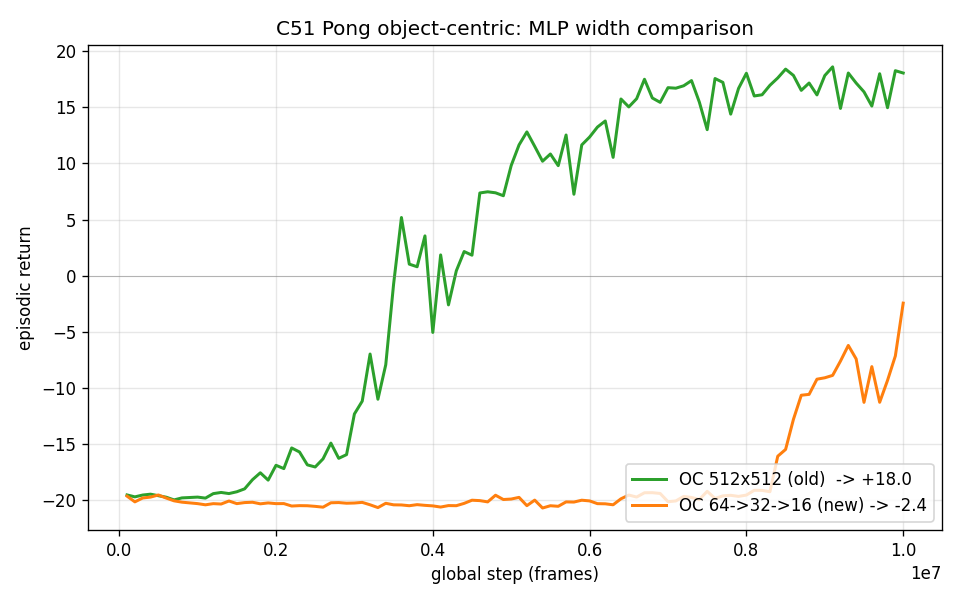
\includegraphics[width=0.78\linewidth]{c51_oc_width_comparison.png}
\caption*{\small Object-centric learning curves overlaid. Old $512\times512$ (green) takes off
at $\sim\!2$M and plateaus at $+18$ by $\sim\!6$M; new $64\to32\to16$ (orange) is flat until
$\sim\!8.3$M, then a steep, unfinished climb to $-2.4$ at 10M.}
\end{figure}

\textbf{Why it got worse.} It is a convergence-\emph{speed} gap, not a capability gap. The
narrow net has far fewer parameters, so it needs many more gradient steps before the value
function is accurate enough to produce a useful greedy policy (hence the $\sim\!8$M stuck
phase). The tightest spot is the final $16$-unit layer feeding the distributional head
($\text{action\_dim}\times n_{\text{atoms}} = 6\times51 = 306$ outputs): a $16\to306$
bottleneck is severe (even CleanRL's CartPole C51 uses $(120,84)$). The new net is also
deeper \emph{and} narrower, which trains more slowly without residual connections.

\textbf{Takeaway.} Normalization---not width---was the real fix for the original OC collapse:
even this tiny net learns. But width buys convergence speed within a fixed budget. We therefore
recommend a middle ground (e.g.\ \texttt{128\,$\to$\,64\,$\to$\,32}, smaller than $512^2$ but
without the $16$-unit bottleneck), or re-running \texttt{64\,$\to$\,32\,$\to$\,16} at 15--20M
frames purely to document the speed cost.

\end{document}
